\section{Introduction}

\subsection{Présentation du projet}

Le COPEVUE a lancé un appel d'offre dans le cadre de la réalisation d'un système de monitoring de sites isolés. Il s'agit donc de concevoir en premier lieu une solution technique permettant de répondre au mieux aux exigences fonctionnelles et non fonctionnelles que le COPEVUE formule. De façon synthétique notre équipe va proposer une solution permettant de surveiller des sites naturels difficiles d'accès (souvent à cause des conditions environnementales) et peu peuplés. Dans ces sites isolés sont souvent regroupés des postes de travail et ces zones doivent pouvoir être surveillées en dépit de la distance qui les sépare du bureau de contrôle.

\subsection{Présentation du document}

Ce document permet de définir précisément l'architecture applicative et technique de l'ensemble de notre solution, en rapport avec le dossier de Spécification Technique des Besoins. L'objectifs est d'apporter une réponse claire aux questions suivantes:

%Copier coller du doc de Regis
\begin{itemize}
	\item Quels sont les objets manipulés?
	\item Quelles sont les données manipulées?
	\item Analyse transformationnelle de ces données
	\item Description des stations locales et du système central
	\item Dimensionnement
	\item Analyse de la complexité
\end{itemize}

\section{Organisation générale du système}

\begin{figure}[hb]
  \centering
  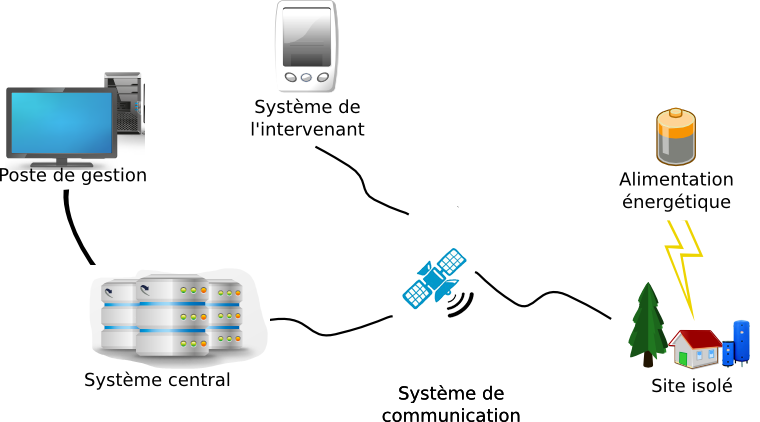
\includegraphics[width=15cm]{schema_architecture_generale_h4111_bis.png}
  \caption[Schéma de l'architecture globale]%
  {Schéma de l'architecture globale}
\end{figure}

\subsection{Système sur site isolé}

Chaque site isolé dispose d'un système complet de monitoring du site, qui est décomposé de la manière suivante :

Les cuves à monitorer sont chacunes équipées de capteurs relevant leur niveau de remplissage. Chaque capteur est géré par un composant connecté direcement dessus, que nous appelerons ici le ``système de gestion du capteur''. Ces systèmes fonctionneront ponctuellement, se réveillant de manière périodique pour effectuer des mesures à l'aide du capteur.

Le site est pourvu d'une ``station centrale'', principalement constituée d'un système embarqué à base d'OS Linux, qui va pouvoir communiquer avec les systèmes de capteurs vu précédement à l'aide d'une connexion sans-fil ZigBee. La station centrale aura elle aussi un fonctionnement ponctuel, se réveillant par tranches de 10 minutes toutes les 6 heures (configuration par défaut, paramétrable bien évidement). Chaque fois qu'un système de gestion de capteur aura effectué une mesure, il essayera d'en communiquer le résultat à la base. En cas d'échec, il sera à même de conserver ces informations en vue d'une transmission ultérieur.\\
C'est un sous-système de la station centrale, le ``système de gestion du site'' qui sera responsable de la collecte des données auprès des capteurs, du maintient de la configuration de la station, mais aussi de la journalisation de données aussi bien logiques que physiques telles que les erreurs systèmes, la température extérieur, etc.

La station centrale dispose d'un autre sous-système, le ``système de transmission'', qui servira quant à lui à la communication avec le système central décrit plus loin. Cette transmission se fera de manière périodique, à une fréquence paramétrable, par satellite ou en utilisant le réseau GSM. Elle permettra d'envoyer dans un sens les relevés des capteurs, et dans l'autre l'envoi de nouveaux paramètres de configuration à la station (et par extension, aux systèmes de gestion de capteurs).

\subsection{Système central}

Le ``système central'' est une application connectée à internet servant à centraliser les informations collectées sur l'ensemble des sites d'un territoire (voir même du monde). En voici le fonctionnement :

Les systèmes de transmission des sites isolés vont communiquer par internet avec le système central pour lui transmettre les derniers relevés des capteurs du site. Celui-ci va alors les stocker en base de données et vérifier si de nouvelles informations de configuration sont disponibles pour ce site. Si c'est le cas, celles-ci seront transmises en réponse.

En arrière plan, le système central va appliquer un ensemble de règles configurables pour vérifier si les nouvelles valeurs transmisent doivent déclencher des actions automatisées telles que des alertes ou des demandes d'intervention sur site.

Le système central va aussi présenter une interface de gestion aux gestionnaire et clients du système, leur permettant de vérifier l'état et l'historique des mesures de chaque site, et la reconfiguration de ceux-ci. Cette interface doit aussi leur permettre de consulter d'éventuelles alertes, et de pouvoir y réagir en planifiant des interventions.

\subsection{Communication}

La communication entre la station et le central s’effectuera la plupart du temps en GSM. La plupart des sites isolés peuvent capter un signal, le GSM permet donc d’avoir une solution efficace, économe et peu cher. Dans le cas où aucune connexion GSM ne peut être faite, la base se connecte via satellite. La couverture des fournisseurs est quasi-totale, ce qui permet d’atteindre toutes les régions isolées. 

La communication entre les modules de capteurs et la base se fait grâce au protocole ZigBee, qui permet de faire un réseau de plus de 60 000 appareils. Le ZigBee est très économe et le protocole est simple d’utilisation. Les cartes appliquant le ZigBee se paye à quelques dizaines d’euros. 

% \section{Règles de pilotage du système} - 'Dafuq is dat shit!!!11111



\section{Architecture applicative}

Au niveau des capteurs, l'usage de micro-contrôleurs programmables ne nous impose pas d'utiliser un système d'exploitation. Le développement sur ces composants se fera en en C, en utilisant les outils fournis par le constructeur.

Pour le système embarqué de la station, le premier choix à faire est celui de l'OS. Il nous faut pour cela un système petit et fiable, qui doit pouvoir supporter la mise en veille profonde pour des raisons d'économie d'energie. Il doit également supporter les connexions USB et PCIe pour pouvoir communiquer avec les différents périphériques que nous comptons lui ajouter. Le choix s'est donc porté sur Embedded Linux, qui non seulement répond à ces contraintes, mais présente de plus l'avantage d'être gratuit et libre, nous autorisant ainsi à l'adapter à nos besoins tout en n'ajoutant pas de coûts supplémentaires.

Les logiciels que nous développerons sur le système embarqué seront en C/C++ pour des raisons de performances et d'empreinte mémoire.

Concernant le système central, l'usage d'une plateforme de cloud computing est envisagé pour permettre des temps de développement plus court (pas de gestion d'infrastructure à faire) et une garantie d'intégrité plus importante sur les données. Au niveau de l'OS, c'est encore une fois sur Linux que s'est porté notre choix, dans sa version serveur cette fois-ci. N'ayant plus à faire ses preuves dans le monde du serveur, on appréciera encore une fois son aspect gratuit/libre, et sa grande versatilité.

Les différentes composants du système central utiliseront les technologies suivantes :

\begin{itemize}
\item NodeJS pour le serveur d'API responsable de la communication avec les sites isolés. Ayant fait ses preuves dans des applications très demandantes en terme de performances, ce serveur/framework web tire partis de son modèle asynchrone pour utiliser au mieux les ressources à sa disposition. Il est par ailleurs simple à interfacer avec les principaux DBMS du marché.
\item Nous nous servirons de Java pour la partie présentation des données. Le logiciel utilisera l'API décrite dans le dossier correspondant.
\item Le moteur de traitement des règles à appliquer sur les données sera lui aussi développé en Java, technologie plus adaptée que NodeJS aux lourds traitements tout en gardant un interfacage efficace et bien fourni avec les DBMS.
\end{itemize}

\section{Architecture informatique et matérielle}

\subsection{Architecture matérielle}

\paragraph{Maintenance} Le technicien chargé de la maintenance du système est équipé d’un module capable de se connecter à la station. Ce module doit être pourvu d’une prise USB pour relier l’appareil à la station. L’application de maintenance est utilisable sur un ordinateur  ou un matériel plus compact tel qu’un PDA ou un Smartphone. 

\paragraph{Capteur} Le module du capteur est équipé d’une carte contenant le capteur, le module de communication sans-fil et l’alimentation. Le système embarqué résiste aux conditions climatiques et a une très grande autonomie.

\paragraph{Base de la station} La base de la station est équipée du module de communication général  (GSM ou satellite selon la localisation du site), d’un module de communication ZigBee pour superviser le reste de la station. Cette base est capable d’enregistrer les informations les plus pertinentes avant de les retransmettre au central. La base est reliée à une source d’énergie qui l’alimente pendant de longue période. 

\subsection{Architecture informatique}

\paragraph{Module capteur} Le module capteur regroupe plusieurs parties logiciels. Le logiciel principal permet de vérifier le niveau de la batterie, de communiquer grâce au module ZigBee et de relever les valeurs du capteur. Pour cela un pilote est implémenté pour assurer une bonne intégration entre les éléments

\paragraph{Base de la station} La base est composé que d’un seul logiciel, qui a pour rôle de superviser la station. Elle doit ainsi relever les valeurs de tous les capteurs, les enregistrer et les retransmettre au central. Ce logiciel peut également reconfigurer différents éléments de la base telle que la période de réveil du système. Le protocole de communication implémenté est sécurisé, pour empêcher une interception des données ou une intrusion dans le système.

\section{Réflexions sur les données}

\subsection{Modèles de données du système}

La question s'est rapidement posée sur la flexibilité que nous voulions apporter à notre modèle de données. En effet, on peut facilement imaginer que le système aura à évoluer à l'avenir selon les fonctionnalités que l'on voudra lui apporter, et le schéma de données du système sera naturellement amené à s'adapter à ces évolutions. Il faut donc nous assurer dès maintenant que cette transition à venir pourra se faire sans problèmes.

Cela peut se traduire par plusieurs règles à respecter lors du développement de certains parties du système. Il a déjà été mentionné auparavant qu'une architecture en couches sera nécessaire pour garantir la maintenabilité du système, et on peut peut rajouter à cela la contrainte de pouvoir régénerer automatiquement la couche DAO des différents composants du système lors d'une modification du schéma de la base de données. Dans le même esprit, on peut aussi imaginer que l'interface d'édition des différents objets métier puisse se construire à la volée en fonction des propriétés de ceux-ci.

C'est évidement une des contraintes dont nous avons du tenir compte lors du choix du DBMS à utiliser. Il fallait en effet que celui-ci puisse supporter des modifications de schéma en temps réel, sans que cela n'ai d'impact sur les performances de celui-ci, et même qu'il puisse accepter plusieurs versions en paralèlle d'un même schéma.

Pour ce qui est de notre premier modèle à proprement parler, nous avons privilégiés une forte resseblance entre notre modèle de données et les objets physiques correspondants à ces entités. Cela présente l'avantage de pouvoir mieux communiquer le sens de notre modèle à des personnes exterieurs au projet, et de permettre des évolutions plus simples à l'avenir, puisque celles-ci seront calquées sur les ajout réels, physiques et concrets qui seront fait au système.

\subsection{Volume de données}

La première problématique qui se pose en regard du volume des données que nous allons devoir gérer est celle de la transmission de celles-ci depuis les sites jusqu'au serveur central. Les progrès récents en terme de transmission de données, autant par satellite que par réseau GSM, assurent un débit d'au moins 128kbps où que l'on se trouve dans le monde. Cela a pour conséquence de ne pas imposer de contrainte forte sur la taille des données que l'on souhaite transmettre. En effet, étant donné la nature de celles-ci, des valeurs de remplissage de cuves, au nombre d'une centaine par site au maximum, sur une période d'une journée (dans le cas où l'on souhaiterais une transmission quotidienne), on peut affirmer que chaque ``fichier'' envoyé par une station fera moins d'un MO. Les envoi étant effectués rapidement, c'est autant d'énergie qui sera économisée, augmentant ainsi la durée d'autonomie de chaque site.

L'autre aspect de la volumétrie des données est celle du stockage de l'historique des relevés de chaque site, et ce sur une longue période, pour être capable de les utiliser plus tard (e.g pour faire une comparaison des moyennes mensuelles d'une année à l'autre). Mais encore une fois, la nature des données concernée, et leur quantité, ne font pas de leur stockage une des principales difficultés de ce système, et un simple déploiement de serveurs SQL feront sans problème l'affaire.

\section{Gestion des problèmes et anomalies, sécurité}

Comme nous l'avons vu, la disponibilité du système est primordiale pour assurer une surveillance efficace des sites, c'est pourquoi il faut se prémunir contre les erreurs et surtout pouvoir gérer celles qui surviendraient pour éviter de paralyser tout le système. Notre architecture modulaire permet de limiter les risques, tous les éléments n'étant pas nécessaire au fontionnement de l'ensemble.
Dans l'architecture, la détection de problèmes matériels est également prévu, avec la possibilité de récupérer l'état des capteurs et autres composants, ce qui permet d'identifier l'origine des erreurs.
Le point névralgique de notre système est le dispositif de communication, son bon fonctionnement est primordial pour tous les autres composants qui gravitent autour. Il faut donc s'assurer de la qualité de service que l'opérateur choisi peut garantir. De notre côté, un soin tout particulier sera porté sur la résilience aux erreurs de ce module, pour ne pas pénaliser la bonne supervision des sites.
Un autre point important est le serveur central, qui matériellement ne présente que peu de risque, grâce au solution de Cloud Computing, par contre il faudra là aussi portée une grande attention à son comportement en cas d'erreur. Au niveau de la base de données, il est possible d'avoir des moyens de retours en arrière (rollback) en cas de corruption de celle-ci.

\newpage
\appendix
\appendixpage

\section{Répresentation informatique des objets}
	
On va lister ici les principaux objets qui seront manipulés par notre solution, sans pour autant fournir une liste exhaustive permettant de constituer la base de données.
On distinguera les principaux objets:

\begin{itemize}
\item capteurs (ID, type )
\item stations (ID, localisation)	
\item relevé des capteurs (ID, ensemble des valeurs horodaté en JSON)
\item PDA (ID, propriétaire, localisation)
\item ordre de maitenance (ID, station_ID, heure )
\item configuration des capteurs (ID, ensembles des paramètres)
\item configuration des stations (ID, ensembles des paramètres)
\item utilisateur (ID, permission)
\end{itemize}

\section{Démarrage du système}

Le démarrage du système, dans notre cas, profite de la contrainte de fiabilité que nous avons prise en compte dans l'ensemble des spécifications des différents sous-systèmes. En effet, il est prévu que les systèmes puissent reprendre leur fonctionnement normal suite à un défaut de leur matériel ou d'un autre système. Nous allons voir ici que cela a pour effet de faciliter la phase de démarrage du système.

La première étape de démarrage du système consiste à mettre sous tension la station centrale ainsi que les différents capteurs. Ceux-ci vont automatiquement essayer de se connecter à la première station qu'il trouveront, et seront ensuite configurable à partir de celle-ci. Pour la station, le système de gestion du site va démarer immédiatement après l'OS, et ce sera à lui de démarer ensuite le système de transmission quand il le jugera utile. Une configuration initiale sera nécéssaire à partir d'un ordinateur connecté directement dessus pour lui renseigner son identifiant et son nom, l'adresse du système central, les informations nécéssaires à l'utilisation du module de transmission (fréquences satellite, code pin de la carte SIM pour ls GSM, etc.) et autres paramètres telle que la granularité avec laquelle doivent être effectuées les mesures pour les différentes types de capteurs, mais aussi la fréquence des transmissions au système central.

Une fois la station centrale configurée, celle-ci commencera automatiquement à accepter les connexion des système de gestion des capteurs, et configurera alors automatiquement ceux-ci. Arrivé à ce stade-là, il n'est pas forcément nécéssaire que le système central soit déjà accéssible. Dans le cas où la station centrale n'arriverait pas à joindre celui-ci, elle conservera les données qu'elle souhaitait lui transmettre, et recommencera plus tard.

Pour ce qui est du système justement, étant donné qu'il s'agit ici d'une application hébergée censée être disponible en permanence, on ne devrait avoir à la démarer qu'une seule fois, en début de l'exploitation.

On constate donc que le fait d'avoir une architecture découplée, et permettant la reprise sur défaut, nous facilite ici la tâche pour ce qui est du démarrage du système.